\documentclass{wileySix}
\usepackage{w-bookps}

% \usepackage{mathptmx}

\usepackage{graphicx}
\usepackage{enumitem}

\setcounter{secnumdepth}{3}

\setcounter{tocdepth}{2}

\begin{document}

\booktitle{Sistem Operasi}
\subtitle{Semua Tentang Sistem Operasi}

\author{Rolly Maulana Awangga}

\halftitlepage
\titlepage



\offprintinfo{Sistem Operasi, pre-release}{Rolly Maulana Awangga}


\begin{copyrightpage}{2018}
Web Service / Rolly Maulana Awangga
\end{copyrightpage}


\dedication{For my family}

\contentsinbrief %optional
\tableofcontents
\listoffigures %optional
\listoftables  %optional

%%%%%%%%%
%%Content 
%%%%%%%%%

\part[Pengenalan Sistem Operasi]
{Pengenalan\\ Sistem Operasi}

\chapter[Contoh]
{Contoh\\ Latex}
\prologue{The sheer volumne of answers can often stifle insight...The purpose
of computing\index{computing!the purpose} is insight, not numbers.}
{Hamming}

\section{Definisi}
Sistem Informasi Geografis merupakan penggalan kata dan Sistem Informasi dan Geografis. Geografis dipandang sebagai bentukan dari geospasial.
Geospasial memiliki arti geo yang berarti bumi dan spasial yang berarti ruang atau keruangan. Jadi geospasial merupakan ilmu yang mempelajari 
tata ruang dari bumi. Tata ruang melingkupi letak suatu titik di bumi baik itu letak kota, provinsi atau negara. Tata ruang juga menyajikan gambaran dari ruang tersebut yang disebut dengan ilmu kartografi atau sering disebut sebagai ilmu pembuatan peta\cite{awangga2017colenak}.

\section{Sejarah Peta}
Perkembangan peta dunia tidak luput dari para ahli geografi dan kartografi. Peta dunia yang populer pada saat ini merupkan kontribusi dari para 
pembuat peta sebelumnya

\subsection{Ptolemy's}
Ptolemy's diduga membuat peta pada abad ke 2


\subsection{Muhammad al-Idrisi}
Seorang ahli geografi dan kartografi Muhammad al-Idrisi membuat peta dunia pada abad ke 11

\begin{figure}[ht]

\centerline{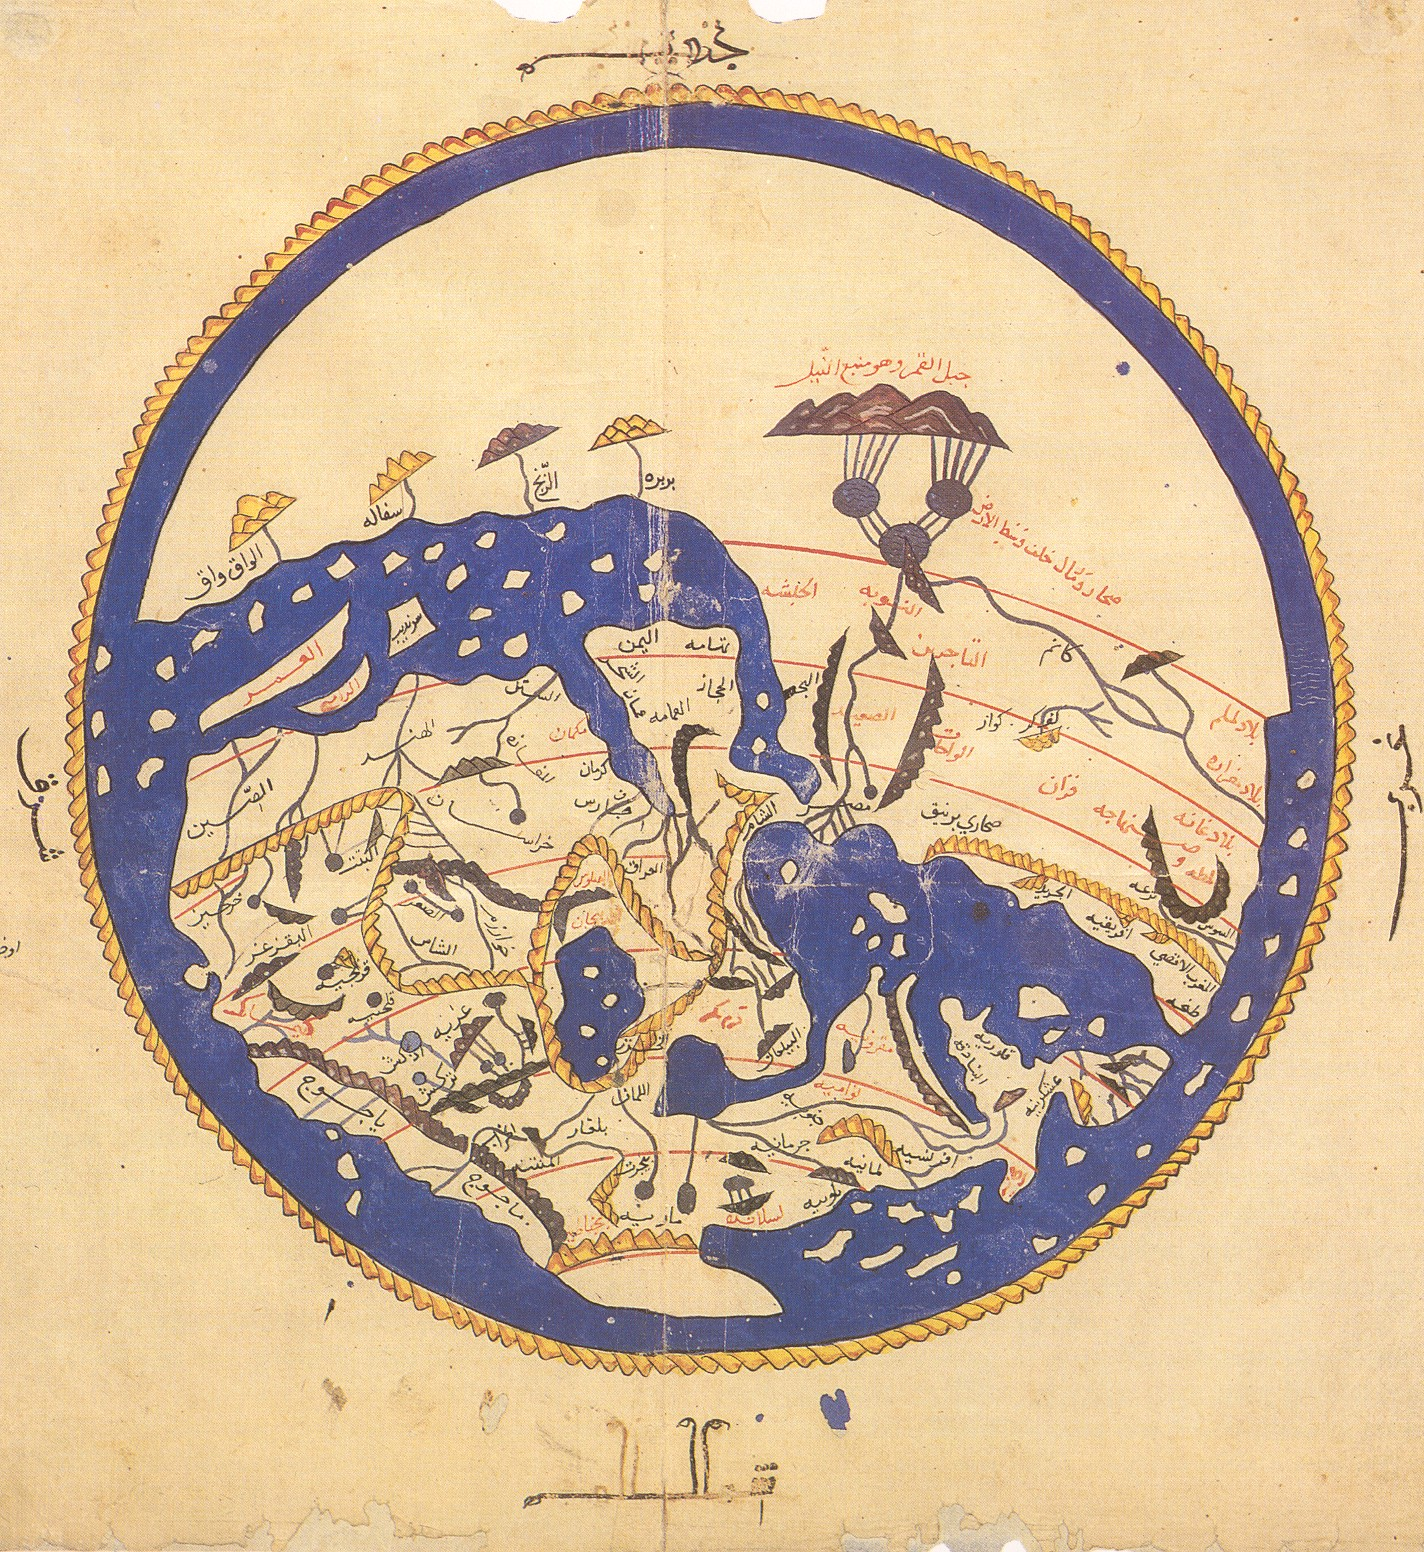
\includegraphics[width=1\textwidth]{figures/petaduniaalid.JPG}}
\caption{Gambaran pengantar peta dunia karya al-Idrisi tahun 1154.}
\end{figure}

\begin{figure}[ht]
	\centerline{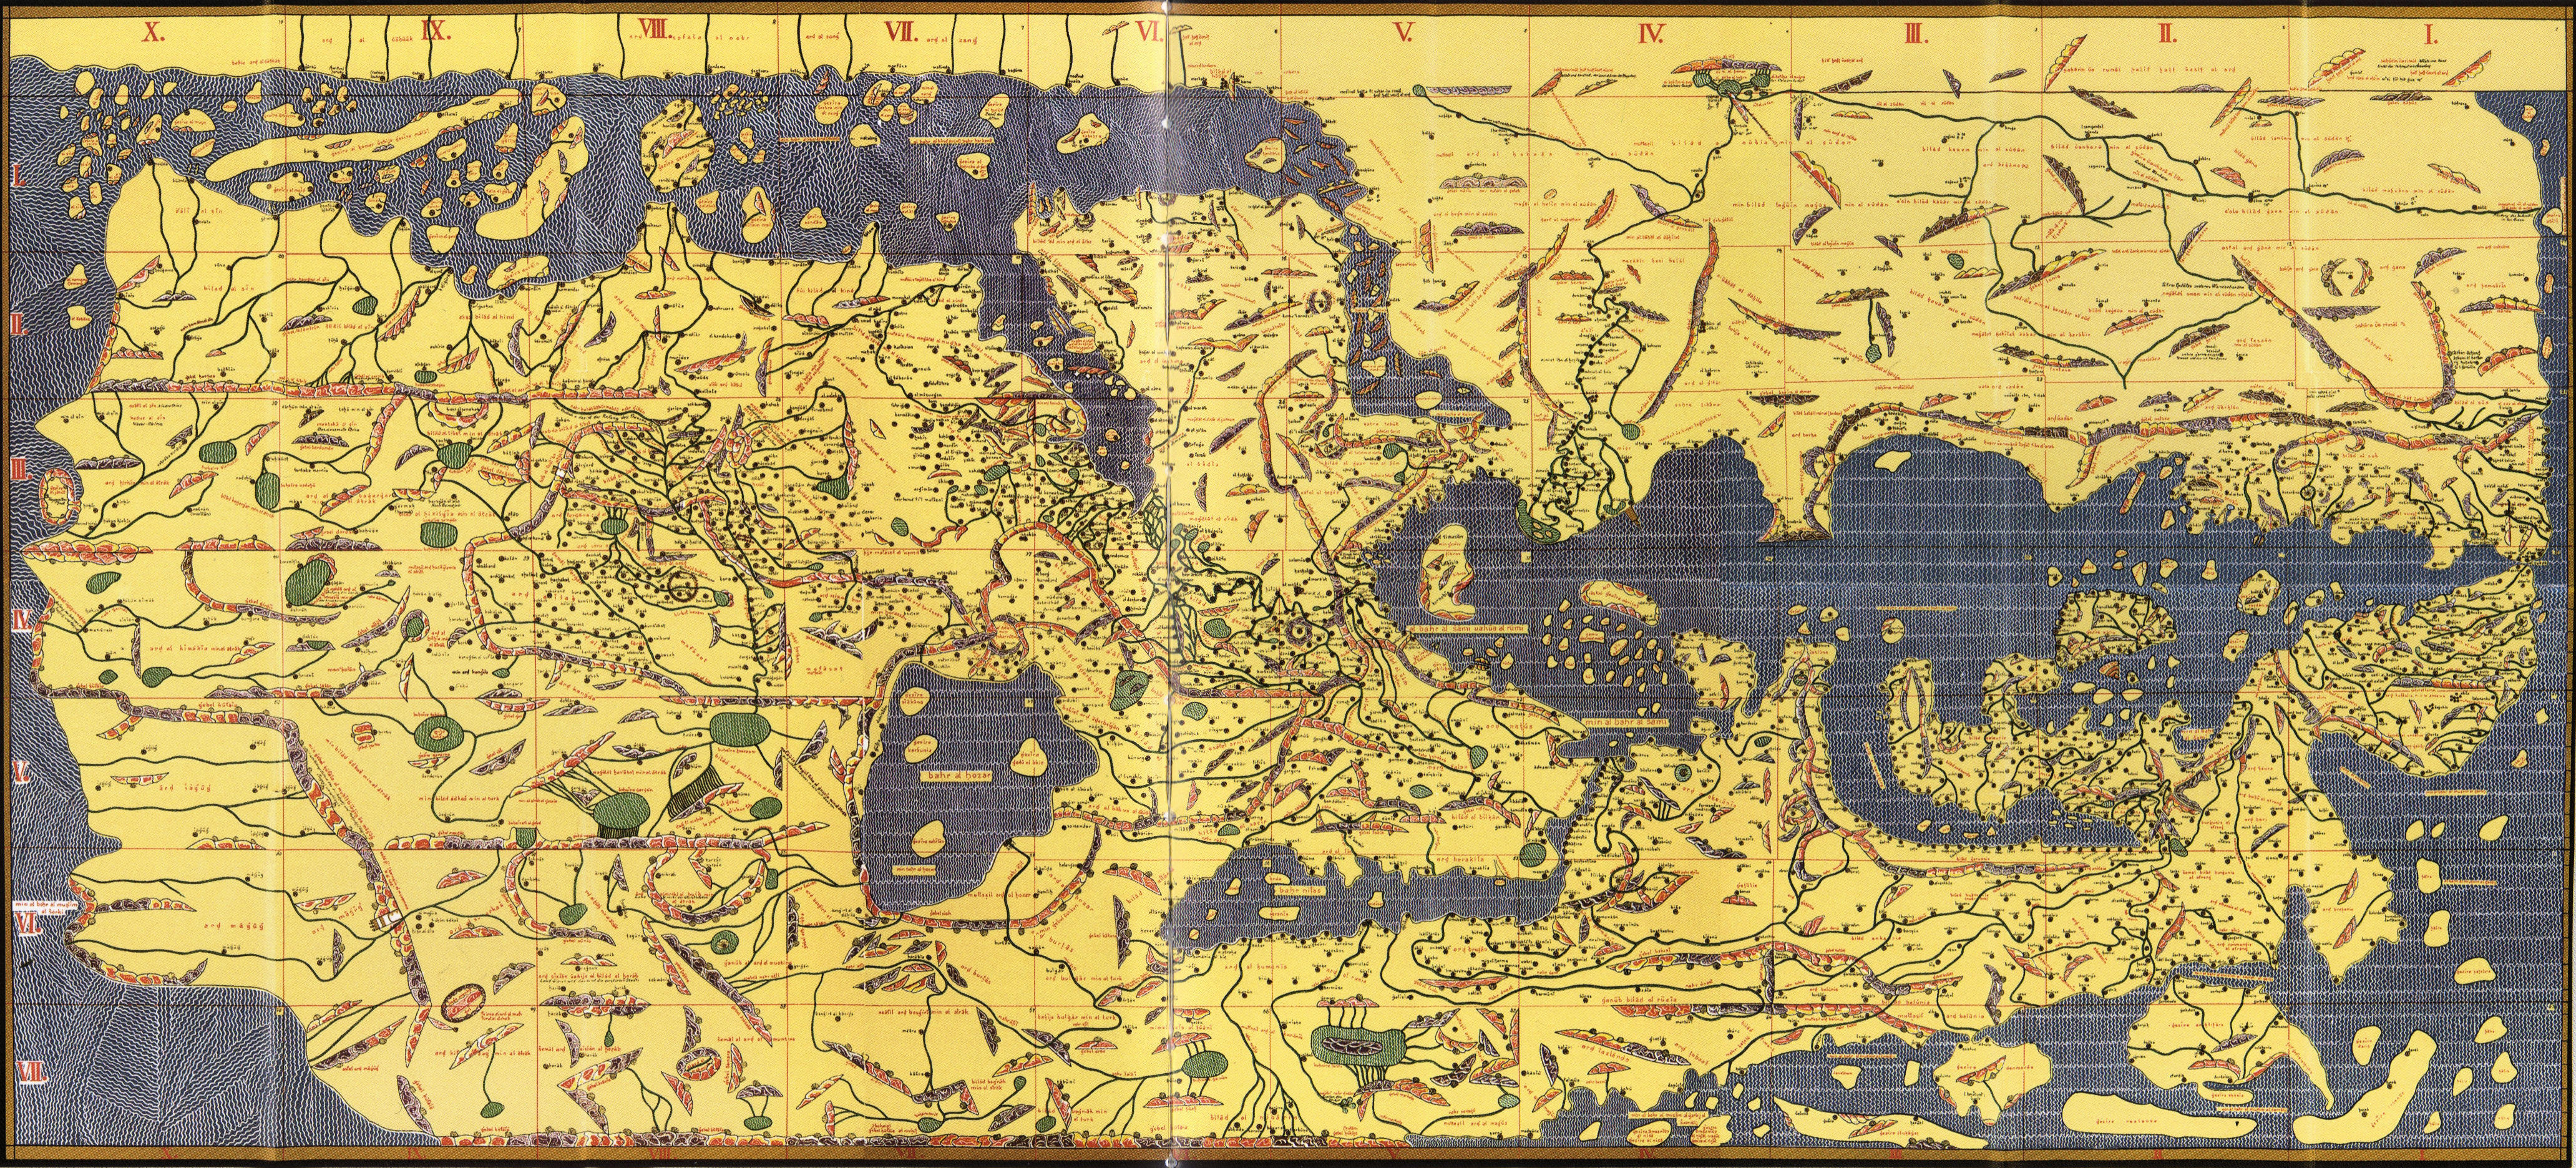
\includegraphics[width=1\textwidth]{figures/TabulaRogeriana.jpg}}
\vskip2pt
\caption{Tabula Rogeriana digambar oleh Al-Idrisi pada tahun 1154 untuk Raja Normandia Roger II dari Sisilia, setelah delapan menetap di istananya, di mana dia bekerja untuk penjelasan dan ilustrasi peta.}
\end{figure}

\section{Penentuan Kordinat}
Kordinat digunakan untuk mengacu sebuah titik lokasi di muka bumi, adapun beberapa jenis standar kordinat yang digunakan adalah.

\subsection{Kordinat Internasional}
Kordinat internasional dikenal dengan long dan lat.


\subsection{Kordinat Indonesia}
Masih ingatkah pelajaran geografi tentang letak Indonesia? maka kita bisa melihat jawaban tersebut dalam kordinat berbahasa indonesia.


%\chapter[Semaphore]
%{Definisi\\ Semaphore}
%\section{System Operasi Semaphore}

	\subsection{Definisi}
	
		\begin{figure}[ht]
			\centerline{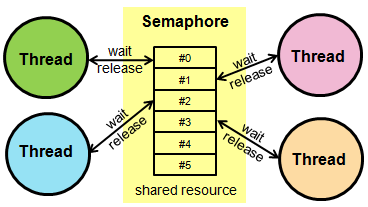
\includegraphics[width=0.5\textwidth]{figures/sema.png}}
			\caption{Semaphore}
			\label{sema}
			\end{figure}
	
		Semaphore merupakan salah satu teknik sinyal pada OS yang paling sederhana, dan merupakan konsep yang penting dalam OS desain, di mana nilai integer digunakan untuk memberi sinyal antar proses. 
		Hanya tiga operasi yang mungkin dilakukan pada semaphores, yang semuanya adalah atom: inisialisasi, keturunan, dan peningkatan. 
		Pengurangan operasi dapat menyebabkan proses yang diblokir, dan peningkatan operasi yang sedang berlangsung dapat mengakibatkan pemblokiran suatu proses. 
		Semaphore pada system operasi merupakan sebuah variabel bertipe integer. Di kehidupan nyata, semaphore merupakan sistem sinyal yang digunakan untuk memberi sinyal atau tanda dan berkomunikasi secara visual. 
		Semafor juga merupakan struktur data dalam bahasa komputer yang digunakan untuk menyinkronkan suatu proses, yaitu untuk memecahkan masalah di mana masalahnya lebih dari satu proses atau bisa 
		seperti thread yang akan dijalankan secara bersamaan dan harus diatur urutan kerja. Semaphore dibuat oleh Edsger Dijkstra dan pertama kali digunakan dalam sistem operasi.
		Nilai semaphore diinisialisasi dengan jumlah sumber daya yang dikontrol oleh pengguna. Dalam kasus khusus di mana ada sumber daya bersama, semaphore disebut semaphore biner. 
		Semaphore adalah solusi klasik dari dining philosophers problem, meskipun itu tidak mencegah deadlock.
		Pada software semaphore, semaphore merupakan variabel yang bertipe data integer tetapi tidak termasuk pada data yang sedang dilakukan inisialisasi, yang hanya dapat diakses melalui dua operasi standar, yaitu increment dan decrement. 
		Semaphore bisa digunakan untuk menyelesaikan masalah sinkronisasi secara umum, berdasarkan jenisnya. Semaphore hanya memiliki nilai 1 atau 0, atau lebih dari sama dengan 0. 
		Konsep semaphore pertama kali diajukan idenya oleh Edsger Dijkstra pada tahun 1967. Semaphore memiliki dua jenis, yaitu, Biner semaphore dan counting semaphore. 
		Biner semaphore tidak bisa memiliki semua jenis integer tetapi hanya memiliki 2 nilai yaitu 1 atau 0, Sering juga disebut sebagai semaphore primitive. Sedangkan Counting semaphore memiliki nilai 0, 1, sampai seterusnya atau integer lainnya. 
		Banyak sistem operasi yang tidak secara langsung menggunakan semaphore jenis ini, namun lebih banyak yang memanfaatkan semaphore jenis biner semaphore. 
		Pada semaphore ini harus diketahui bahwa, ada beberapa jenis dari counting semaphore yang salah satu jenisnya adalah semafor yang tidak bisa mencapai nilai negatif dan jenis yang lain adalah semaphore yang dapat mencapai nilai negatif. 
		Solusi dari Pembuatan Counting Semaphore adalah Binary Semaphore. Pembuatan counting semaphore banyak dilakukan para programmer untuk memenuhi alat sinkronisasi yang sesuai dengannya. 
		
		Operasi standarnya dalam bahasa pemrograman C :
		
		\begin{verbatim}
			void kunci(int sem_value) {
				while(sem_value <= 0);
				sem_value�;
			}
			void buka(int sem_value) {
				sem_value++;
			}
		\end{verbatim}
		
	\subsection{Prinsip Semaphore}
	
		\begin{enumerate}

			\item Suatu proses yang berbeda bisa berkaitan dengan memanfaatkan sinyal - sinyal.
			\item Suatu proses dapat dihentikan oleh proses yang lain.
			\item Semaphore bertipe data integer yang diakses oleh dua operasi atomik standar (wait dan signal).
			\item Ada dua operasi di semaphore (Down dan UP). Yang nama aslinya : P dan V.
		
		\end{enumerate}

	\subsection{Kelemahan Semaphore}
	
		\begin{enumerate}

			\item Semaphore termasuk Low Level.
			\item Dikarenakan semaphore tersebar di dalam seluruh program maka kita akan kesulitan dalam pemeliharaannya.
			\item Jika kita menghapus \"wait\" akan mengakibatkan \"nonmutual exclusion\".
			\item Jika kita menghapus \"signal\" akan mengakibatkan \"deadlock\".
			\item Jika terjadi deadlock akan sulit untuk dideteksi.

		\end{enumerate}
		
	\subsection{Semantik dan Impelementasi}
		Menghitung semaphores dilengkapi dengan dua operasi, secara historis dilambangkan sebagai P dan V (lihat § Nama operasi untuk nama alternatif). 
		Operasi V menambahkan semaphore S, dan operasi P menurunkannya.

		Nilai semaphore S adalah jumlah unit sumber daya yang saat ini tersedia. Operasi P membuang waktu atau tidur sampai sumber daya yang dilindungi oleh 
		semaphore menjadi tersedia, pada saat itu sumber daya segera diklaim. Operasi V adalah kebalikannya: ia membuat sumber daya tersedia lagi setelah proses
		selesai menggunakannya. Satu properti penting dari semaphore S adalah bahwa nilainya tidak dapat diubah kecuali dengan menggunakan operasi V dan P.

		Cara sederhana untuk memahami operasi tunggu (P) dan sinyal (V) adalah:
		
		\begin{itemize}
		
			\item menunggu: Jika nilai variabel semaphore tidak negatif, turunkan dengan 1. Jika variabel semaphore sekarang negatif, proses menunggu eksekusi 
			      diblokir (yaitu, ditambahkan ke antrian semaphore) sampai nilainya lebih besar atau sama dengan 1 Jika tidak, proses terus berjalan, setelah 
				  menggunakan satu unit sumber daya.
			\item sinyal: Menambah nilai semaphore variabel dengan 1. Setelah kenaikan, jika nilai pre-increment negatif (berarti ada proses menunggu sumber 
				  daya), ia mentransfer proses yang diblokir dari antrian menunggu semaphore ke antrean siap.
			
		\end{itemize}
		
		Banyak sistem operasi menyediakan primitif semaphore yang efisien yang membuka blokir proses menunggu ketika semaphore bertambah. Ini berarti bahwa proses tidak membuang waktu untuk memeriksa nilai semaphore yang tidak perlu.Konsep penghitungan semaphore dapat diperpanjang dengan kemampuan untuk mengklaim atau mengembalikan lebih dari satu \"unit\" dari semaphore, teknik yang diterapkan di Unix. Operasi V dan P yang dimodifikasi adalah sebagai berikut, menggunakan tanda kurung siku untuk menunjukkan operasi atom, yaitu operasi yang tampak terpisah dari perspektif proses lain:

		Semaphore pada system operasi merupakan sebuah variabel bertipe integer. Di kehidupan nyata, semaphore merupakan sistem sinyal yang digunakan untuk memberi sinyal atau tanda dan berkomunikasi secara visual. PPada software semaphore, semaphore merupakan variabel yang bertipe data integer tetapi tidak termasuk pada data yang sedang dilakukan inisialisasi, yang hanya dapat diakses melalui dua operasi standar, yaitu increment dan decrement. 
		Semaphore bisa digunakan untuk menyelesaikan masalah sinkronisasi secara umum, berdasarkan jenisnya. Semaphore hanya memiliki nilai 1 atau 0, atau lebih dari sama dengan 0. Konsep semaphore pertama kali diajukan idenya oleh Edsger Dijkstra pada tahun 1967. Semaphore memiliki dua jenis, yaitu, Biner semaphore dan counting semaphore. Biner semaphore hanya memiliki nilai 1 atau 0, Sering juga disebut sebagai semaphore primitive. Sedangkan Counting semaphore memiliki nilai 0, 1, sampai seterusnya atau integer lainnya. Banyak sistem operasi yang tidak secara langsung menggunakan semaphore jenis ini, namun lebih banyak yang memanfaatkan semaphore jenis biner semaphore

	
	\subsection{Prinsip Semaphore}
		\begin{enumerate}

			\item Suatu proses yang berbeda bisa berkaitan dengan memanfaatkan sinyal - sinyal.
			\item Suatu proses dapat dihentikan oleh proses lainnya.
			\item Semaphore bertipe data integer yang diakses oleh dua operasi atomik standar (wait dan signal).
			\item Ada dua operasi di semaphore (Down dan UP). Yang nama aslinya : P dan V.
			
		\end{enumerate}
		
	\subsection{Kelemahan Semaphore}

		\begin{enumerate}

			\item Semaphore termasuk Low Level.
			\item Dikarenaka semaphore tersebar di dalam seluruh program maka kita akan kesulitan dalam pemeliharaannya.
			\item Jika kita menghapus \"wait\" akan mengakibatkan \"nonmutual exclusion\".
			\item Jika kita menghapus \"signal\" akan mengakibatkan \"deadlock\".
			\item Jika terjadi deadlock akan sulti untuk dideteksi.
			
		\begin{enumerate}
		
	\cite{luu1982apparatus}
	\cite{lauesen1975large}
	\cite{hoare1974monitors}


\chapter[Internet]
{Definisi\\ Internet}
%Nama Kelompok: Sistem_Operasi_Deadlock
%Kelas: D4 TI 1B
%Alit Fajar Kurniawan(1174057) 
%Muhammad Iqbal Panggabean(1174063)
%Muhammad Afra Faris(1174041)
%Khadijah Hasanah Puteri Harahap(1174044)

\section {DEADLOCK}

\subsection {Deadlock}
\subsubsection {Pengertian Deadlock}
	Pada kesempatan ini saya akan menjelaskan tentang definisi Deadlock, Deadlock ialah suatu keadaan yang dimana dua proses atau lebih, saling menunggu proses untuk dapat melepaskan sumber daya yang sedang dijalankan. Misalnya proses A yang memperlukan suatu sumber daya, tetapi sumber saya tersebut sedang digunkana oleh proses lain. Untuk lebih paham mengenai pengertian dari deadlock dan bagaimana cara mengatasinya, anda dapat membandingkannya dengan situasi yang satu ini. Pertama, Dalam kehidupan kita tentu membutuhkan suatu pekerjaan, dan untuk memperoleh suatu pekerjaan, anda harus memiliki pengalaman yang baik, untuk dapat memiliki pengalaman yang baik anda harus bekerja.

	\begin{figure}[ht]
	\centerline{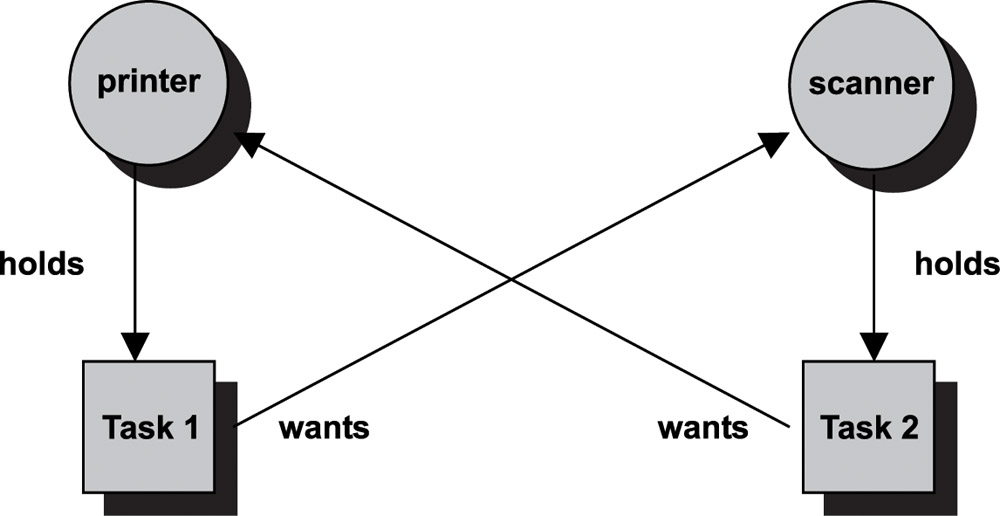
\includegraphics[width=1\textwidth]{figures/deadlock1.jpg}}
	\caption{Gambar Deadlock}
	\label{Gambar}
	\end{figure}
      
      Gambar \ref{Gambar_Deadlock} Contoh gambar pada saat terjadinya deadlock.

\subsection {Masalah Deadlock dan Metode Penanganan Deadlock}
\subsubsection {Masalah Deadlock}
	Deadlock merupakan dampak pengaruh dari sinkronisasi, yaitu dimana satu variabel yang digunakan oleh dua proses yang berbeda. Deadlock selalu tidak terlepas dari yang namanya sumber daya, karena hampir secara keseluruhan merupakan masalah mengenai sebuah sumber daya yang digunakan secara bersamaan. Sebuah Kelompok Proses yang diblok atau diblokir, dimana setiap proses memegang sebuah resource dan kemudian menunggu resource lain dari proses yang berada didalam proses yang sedang diBlok tersebut, biasanya dari semua proses-proses atau resource yang non preemptive.
	
\subsubsection {Metode Penanganan}
	Ada tiga Metode penanganan Deadlock:
	Yang Pertama yaitu, anda harus menggunakan satu protokol yang dapat membuat anda yakin bahwa sistem tersebut tidak akan pernah mengalami kejadian deadlock. Metode ini bisa disebut dengan Deadlock Prevention atau Avoidance.
	
	Yang Kedua, anda harus memberikan izin sistem untuk mengalami kejadian deadlock, namun setelah terjadinya deadlock anda harus dengan cepat segera untuk memperbaiki sistem yang mengalami deadlock tersebut. Metode ini biasanya disebut dengan Deadlock detection and recovery.
	
	Dan yang terakhir, anda hanya mengabaikan semua permasalahan yang terjadi secara bersamaan, dan kemudian menganggap bahwa deadlock tidak akan terjadi, metode ini digunakan dalam berbagai sistem operasi komputer, termasuk windows dan unix.

\begin{table}[H]
\begin{tabular}{|c|c|c|c|c|}
hline
Proses & Jumlah Sumber Daya Digenggam & Maksimum Sumber Daya Dibutuhkan\\
\hline
X   & 2 & 10\\
Y   & 1 & 3\\
Z   & 3 & 7\\
\hline
Tersedia 4
\hline
\end{tabular}
\end{table}

\subsection {Deadlock Detection}
\begin {enumerate}
\item
1. Pendeteksian secara Algoritma, yaitu dengan cara kita mengetahui jika terjadinya deadlock, deadlock terjadi jika suatu permintaan tidak dapat ditangani segera.
	
\item
2. Recovery atau Pemulihan, yaitu yang pertama menggagalkan semua proses deadlock, yang kedua mem backup semua proses yang deadlock dan kemudian silahkan melakukan restart di semua proses yang sedang terjadi, yang ketiga menggagalkan semua proses yang deadlock secara berurutan sehingga tidak akan terjadi lagi deadock, dan yang terakhir yaitu menggagalkan pengalokasian resource secara berurutan hingga tidak ada deadlock.

\end {enumerate}

\subsection {Beberapa hal yang terjadi ketika mendeteksi adanya deadlock}
\begin {enumerate}
\item
1. Permintaan sumber daya dikabulkan selama memungkinkan.
\item
2. Sistem operasi melakukan scanning apakah ada kondisi circular wait secara peiodik.
\item
3. Pemeriksaan dilakukan setiap ada sumber daya yang hendak digunakan.
\item
4. memeriksa dengan algoritma tertentu.
\end {enumerate}

\subsection {Beberapa jalan untuk kembali dari deadlock}
\begin {enumerate}
\item
1. Lewat Preemption, yaitu dengan jauhkan sumber daya dari pemakainya untuk sementara waktu, tujuannya untuk memberikannya pada proses lain. strategi dengan memberikannya kesempatan pada proses lain dengan tanpa diketahui oleh pemilik dari sumber daya itu dan tergantung juga dari sifat sumber daya itu sendiri.
\item
2. Lewat melacak kembali, setelah melakukan prosesn dari preemption tersebut maka secara otomatis proses utama yang diambil sumber dayanya akan stop dan tidak akan melanjutkan prosesnya, oleh karena itu dibutuhkan langkah untuk dapat kembali pada keadaan aman, tetapi untuk menentukan keadaan aman tersebut sangatlah susah.
\item
3. Mematikan proses yang menyebabkan deadlock, ini merupakan cara yang sangat umum digunakan yaitu dengan cara mematikan semua proses yang mengalami deadlock.
\item
4. Menghindari deadlock, pada sistem permintaan untuk sumberdaya biasanya hanya dilakukan sekali saja, sistem harus sudah dapat mengenali bahwa sistem itu aman atau tidak.
\end {enumerate}

\subsection {Reference}

@article{siahaan2015penyelarasan,
  title={Penyelarasan Pada Masalah Dining Philosophers Menggunakan Algoritma Lock \& Release},
  author={Siahaan, Andysah Putera Utama},
  journal={TECHSI-Jurnal Teknik Informatika},
  volume={7},
  number={1},
  year={2015}
}

@article{fauzi2013perangkat,
  title={PERANGKAT LUNAK VISUALISASI PERJALANAN KERETA API DENGAN MENGGUNAKAN PENDEKATAN SEMAPHORE, DEADLOCK SOLUTION DAN ALGORITMA DIJKSTRA},
  author={Fauzi, Esa},
  year={2013},
  publisher={Universitas Widyatama}
}

@book{silberschatz2014operating,
  title={Operating system concepts essentials},
  author={Silberschatz, Abraham and Galvin, Peter Baer and Gagne, Greg},
  year={2014},
  publisher={John Wiley \& Sons, Inc.}
}

\chapter[Starvation]
{Definisi\\ Starvation}
\section{Starvation}
Perkembangan sistem komputer mendatang adalah menuju ke sistem multi-processing, multiprogramming, terdistribusi dan paralel yang mengharuskan adanya proses-proses yang berjalan bersama dalam waktu yang bersamaan. Hal demikian merupakan masalah yang perlu perhatian dari perancang sistem operasi. Kondisi dimana pada saat yang bersamaan terdapat lebih dari satu proses disebut dengan kongkurensi (proses-proses yang kongkuren). Dan dalam kongruensi ini pasti ada masalah yang salah satunya adalah STARVATION.

%\chapter[Backend]
%{Definisi\\ Backend}
%\input{section/1Backend.tex}

%\chapter[Frontend]
%{Definisi\\ Frontend}
%\input{section/1Frontend.tex}

% contoh aplikasi web service
% web service
% protokol
% port

% HTTP
% URL
% POST
% GET


\bibliographystyle{IEEEtran}
\bibliography{references, sumber, starref, bib}

\printindex

\end{document}
